\documentclass[twoside]{article}
\usepackage[utf8]{inputenc}
\usepackage[english]{babel}
\usepackage{amsmath}
\usepackage{graphicx}

\usepackage{anysize}
\marginsize{3 cm}{2.7 cm}{2.7 cm}{2.7 cm}

\begin{document}
\title{4th assignment}
\author{Joaquim Brugués Mora}
\maketitle

{\bf Note:} The code is adaptable for any non-degenerate system, but the integration times have been chosen such that the plots were clear enough. Systems diferent from the examples will run perfectly, but might produce not so nice plots if the integration times are not adapted.

\

Al plots are for a linear system, this means, of the form

$$\dot{x} = A x .$$

For $A = [2,-5;1,-2]$:

\begin{figure}[!ht]
\centering
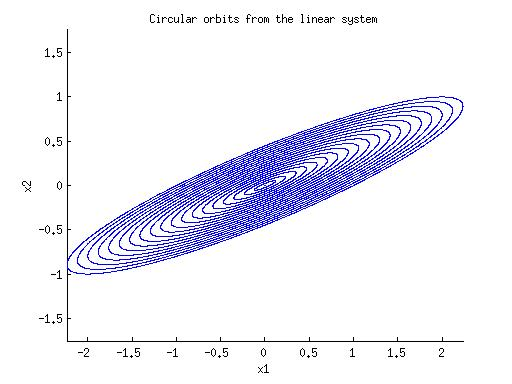
\includegraphics[scale=0.6]{circular.jpg}
\end{figure}

\newpage

For $A = [3,-2;4,-1]$:

\begin{figure}[!ht]
\centering
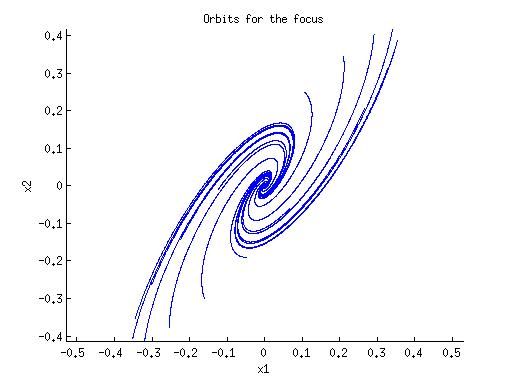
\includegraphics[scale=0.6]{spiral.jpg}
\end{figure}

For $A = [-1,0;3,2]$:

\begin{figure}[!ht]
\centering
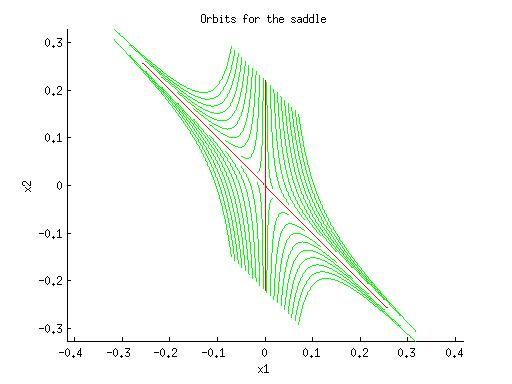
\includegraphics[scale=0.75]{saddle.jpg}
\end{figure}

\newpage

And the MATLAB code:

\begin{verbatim}

clear all
tol = 10^(-12);
number_of_orbits = 20;

fprintf('Input the values of a,b,c,d for a 2x2 matrix A = [a,b;c,d]:\n');
A = input('A: ');

%Compute the eigenvalues and output them.
[V,D] = eig(A);
l1 = D(1,1)
l2 = D(2,2)

%Produce some output descriving the system.
r1 = real(l1); r2 = real(l2);
if (abs(r1)<tol && abs(r2)<tol)
    fprintf('The system has a center at the origin.\n');
else
    if (r1 < 0) 
        if (r2 < 0)
            fprintf('The system has an attractor point at the origin.\n');
        else if (r2 > 0)
                frpintf('The system has a saddle at the origin.\n');
            end
        end
    else
        if (r2 > 0)
            fprintf('The system has a repulsor point at the origin.\n');
        else if (r2 < 0)
                fprintf('The system has a saddle at the origin.\n');
            end
        end
    end
end

%Define the function for the ODE integration at the plots:
F = @(t,x) A*x;
odeoptions = odeset('RelTol',tol,'AbsTol',tol);

figure(1)
hold on
xlabel('x1'); ylabel('x2');
axis equal
%Distinguish two kinds of plots
if (abs(imag(l1)) < tol)
    %The case with stable and unstable manifolds, with a phase portrait.
    if (r2 < 0)
        %We do this trick to have a simpler casuistic. Now we only have
        %r1> 0 or r1 < 0.
        F = @(t,x) -A*x;
        r1 = -r1; r2 = -r2;
    end
    if (r1 < 0)
        %Saddle.
        title('Orbits for the saddle')
        point1_atractor = 10^(-5)*V(:,1);
        point2_atractor = -10^(-5)*V(:,1);
        point1_repulsor = 10^(-5)*V(:,2);
        point2_repulsor = -10^(-5)*V(:,2);
        [~,W11] = ode45(F,[0,-5],point1_atractor,odeoptions);
        [~,W12] = ode45(F,[0,-5],point2_atractor,odeoptions);
        [~,W21] = ode45(F,[0,10.5],point1_repulsor,odeoptions);
        [~,W22] = ode45(F,[0,10.5],point2_repulsor,odeoptions);
        plot(W11(:,1),W11(:,2),'r',W12(:,1),W12(:,2),'r',W21(:,1),W21(:,2),'r',W22(:,1),W22(:,2),'r');
        
        %Finally generate some plots to complete the phase portrait of the
        %system.
        k = linspace(0,1,number_of_orbits);
        point_init1 = W11(end,:)+0.1*V(:,2)';
        point_init2 = W11(end,:)-0.1*V(:,2)';
        point_init3 = W12(end,:)+0.1*V(:,2)';
        point_init4 = W12(end,:)-0.1*V(:,2)';
        for i=1:number_of_orbits
            point1 = (1-k(i))*point_init1 + k(i)*point_init2;
            point2 = (1-k(i))*point_init3 + k(i)*point_init4;
            [~,orbit1] = ode45(F,[0,1.5],point1,odeoptions);
            [~,orbit2] = ode45(F,[0,1.5],point2,odeoptions);
            plot(orbit1(:,1),orbit1(:,2),'g',orbit2(:,1),orbit2(:,2),'g')
        end
    else
        %Node.
        title('Invariant manifolds')
        point1 = 10^(-5)*V(:,1);
        point2 = -10^(-5)*V(:,1);
        point3 = 10^(-5)*V(:,2);
        point4 = 10^(-5)*V(:,2);
        [~,W11] = ode45(F,[0,10],point1,odeoptions);
        [~,W12] = ode45(F,[0,10],point2,odeoptions);
        [~,W21] = ode45(F,[0,10],point3,odeoptions);
        [~,W22] = ode45(F,[0,10],point4,odeoptions);
        plot(W11(:,1),W11(:,2),W12(:,1),W12(:,2),W21(:,1),W21(:,2),W22(:,1),W22(:,2),'r');
    end
else
    %The case with a center or a focus at the origin.
    if (abs(r1) < tol)
        %Circular orbits.
        x0 = linspace(10^(-5),1,number_of_orbits);
        title('Circular orbits from the linear system')
        for i=1:number_of_orbits
            point0 = [x0(i);0];
            [~,yout] = ode45(F,[0,2*pi],point0,odeoptions);
            plot(yout(:,1),yout(:,2),'-o','MarkerSize',0.5)
        end
    else
        %Spirals.
        theta0 = linspace(0,2*pi,number_of_orbits);
        point0 = 10^(-5)*[cos(theta0);sin(theta0)];
        title('Orbits for the focus')
        if (r1 < 0)
            %Integrate backwards, since it's an attractor point.
            for i=1:number_of_orbits
                [~,yout] = ode45(F,[-10,0],point0(:,i),odeoptions);
                plot(yout(:,1),yout(:,2),'-o','MarkerSize',0.5)
            end
        else
            %Integrate onwards in time, it's a repulsor point.
            for i=1:number_of_orbits
                [~,yout] = ode45(F,[0,10],point0(:,i),odeoptions);
                plot(yout(:,1),yout(:,2),'-o','MarkerSize',0.5)
            end
        end
    end
end
\end{verbatim}

\end{document}